% !TEX encoding = UTF-8 Unicode
%%%%%%%%%%%%%%%%%%%%%%%%%%%%%%%%%%%%%%%%%
% Beamer Presentation
% LaTeX Template
% Version 1.0 (10/11/12)
%
% This template has been downloaded from:
% http://www.LaTeXTemplates.com
%
% License:
% CC BY-NC-SA 3.0 (http://creativecommons.org/licenses/by-nc-sa/3.0/)
%
%%%%%%%%%%%%%%%%%%%%%%%%%%%%%%%%%%%%%%%%%

%----------------------------------------------------------------------------------------
%	PACKAGES AND THEMES
%----------------------------------------------------------------------------------------

\documentclass{beamer}

\mode<presentation> {

% The Beamer class comes with a number of default slide themes
% which change the colors and layouts of slides. Below this is a list
% of all the themes, uncomment each in turn to see what they look like.

%\usetheme{default}
%\usetheme{AnnArbor}
%\usetheme{Antibes}
%\usetheme{Bergen}
%\usetheme{Berkeley}
%\usetheme{Berlin}
%\usetheme{Boadilla}
%\usetheme{CambridgeUS}
%\usetheme{Copenhagen}
%\usetheme{Darmstadt}
%\usetheme{Dresden}
%\usetheme{Frankfurt}
%\usetheme{Goettingen}
%\usetheme{Hannover}
%\usetheme{Ilmenau}
%\usetheme{JuanLesPins}
%\usetheme{Luebeck}
\usetheme{Madrid}
%\usetheme{Malmoe}
%\usetheme{Marburg}
%\usetheme{Montpellier}
%\usetheme{PaloAlto}
%\usetheme{Pittsburgh}
%\usetheme{Rochester}
%\usetheme{Singapore}
%\usetheme{Szeged}
%\usetheme{Warsaw}

% As well as themes, the Beamer class has a number of color themes
% for any slide theme. Uncomment each of these in turn to see how it
% changes the colors of your current slide theme.

%\usecolortheme{albatross}
%\usecolortheme{beaver}
%\usecolortheme{beetle}
%\usecolortheme{crane}
%\usecolortheme{dolphin}
%\usecolortheme{dove}
%\usecolortheme{fly}
%\usecolortheme{lily}
%\usecolortheme{orchid}
%\usecolortheme{rose}
%\usecolortheme{seagull}
%\usecolortheme{seahorse}
%\usecolortheme{whale}
%\usecolortheme{wolverine}

%\setbeamertemplate{footline} % To remove the footer line in all slides uncomment this line
%\setbeamertemplate{footline}[page number] % To replace the footer line in all slides with a simple slide count uncomment this line

%\setbeamertemplate{navigation symbols}{} % To remove the navigation symbols from the bottom of all slides uncomment this line
}

\usepackage{graphicx} % Allows including images
\usepackage{booktabs} % Allows the use of \toprule, \midrule and \bottomrule in tables
\usepackage{xeCJK}
\usepackage{color}
\usepackage{listings}
\lstset{numbers=left}
\usepackage{tikz}


%----------------------------------------------------------------------------------------
%	TITLE PAGE
%----------------------------------------------------------------------------------------

\title[Threads]{Threads} % The short title appears at the bottom of every slide, the full title is only on the title page

\author{张海宁} % Your name
\institute[计算机科学与技术学院] % Your institution as it will appear on the bottom of every slide, may be shorthand to save space
{
贵州大学 \\ % Your institution for the title page
\medskip
\textit{hnzhang1@gzu.edu.cn} % Your email address
}
\date{\today} % Date, can be changed to a custom date

\begin{document}

\begin{frame}
\titlepage % Print the title page as the first slide
\end{frame}

\begin{frame}
\frametitle{Overview} % Table of contents slide, comment this block out to remove it
\tableofcontents % Throughout your presentation, if you choose to use \section{} and \subsection{} commands, these will automatically be printed on this slide as an overview of your presentation
\end{frame}

%----------------------------------------------------------------------------------------
%	PRESENTATION SLIDES
%----------------------------------------------------------------------------------------
\section{Threads}
\begin{frame}
\Huge{\centerline{Threads}}
\end{frame}
\subsection{What is a Threads}
\begin{frame}
\Huge{\centerline{What is a Threads}}
\end{frame}
\begin{frame}{Threads}
我们知道可以通过多个进程来执行多任务,但是考虑到进程的资源占用等问题,本章讲解线程来实现多任务操作。

线程是一个程序的多个不同的执行部分,它们共享全局变量。

\end{frame}
\begin{frame}{线程和进程}
\begin{enumerate}
\item
进程是操作系统进行资源(包括cpu、内存、磁盘IO等)分配的最小单位
\item
线程是cpu调度的基本单位
\item
我们打开的微信,浏览器都是一个进程。
进程可能有多个子任务,比如微信要接受消息,发送消息,这些子任务就是线程。
资源分配给进程,线程共享进程资源。
\item
线程的调度比进程的调度所需要的系统开销要小得多。
\end{enumerate}
\end{frame}
%----------------------------------------------------
\subsection{How to create threads}
\begin{frame}
\Huge{\centerline{How to create threads}}
\end{frame}
\begin{frame}[fragile]{线程相关的函数 I}
\begin{block}{函数原型}
\begin{verbatim}
#include <pthread.h>
int pthread_create(pthread_t *thread, pthread_attr_t *attr, 
  void *(*start_routine)(void *), void *arg);
\end{verbatim}
\begin{enumerate}
\item
第一个参数是事先声明的一个pthread类型的指针,新创建的线程通过这个指针来引用。
\item
第二个参数用来设置线程的属性,一般情况下可以设置为NULL。
\item
第三个参数是本线程要执行的具体方法(函数)的指针。
\item
最后一个参数是本线程执行第三个参数指定的方法时,需要使用的参数。
\item
如果创建线程成功会返回0 。
\end{enumerate}
\end{block}
\end{frame}

\begin{frame}[fragile]{线程相关的函数 II}
\begin{block}{函数原型}
\begin{verbatim}
#include <pthread.h>
void pthread_exit(void *retval);
int pthread_join(pthread_t th, void **thread_return);
\end{verbatim}
\begin{enumerate}
\item
pthread\_exit会结束调用它的线程。
\item
pthread\_join是主程序用来等待子线程结束的方法,和进程里的wait类似。
\begin{enumerate}
\item
第一个参数用来指定是哪个线程。
\item
第二个参数用来存储线程的返回值。
\item
如果成功会返回0 。
\end{enumerate}
\end{enumerate}
\end{block}
\end{frame}
\begin{frame}[fragile]{多线程例子}
\begin{verbatim}
void *fmt(void * g);
int main(){
 pthread_t  pth[2];  void * rz;
 char  ch='a';  char  chA='A';
 int ra=pthread_create(&pth[0],NULL,fmt,&ch);
 int rA=pthread_create(&pth[1],NULL,fmt,&chA);
 pthread_join(pth[0],&rz);
 pthread_join(pth[1],&rz);
 printf("two threads has finished.\n");	
}
void *fmt(void * arg){
 char c=*(char *)arg;  int i=0;
 for(char a=c;i<3;a++,i++){
  printf("%c\n",a); sleep(1);}
 return NULL; 
 //pthread_exit("a thread finished.\n");}
\end{verbatim}
\end{frame}
\begin{frame}{执行过程}
\begin{block}{执行示意图}
\center{
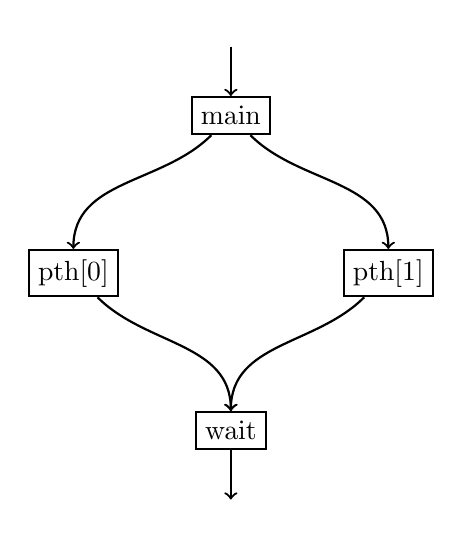
\begin{tikzpicture}
\node (s)at (10,7) {};
\node[draw,rectangle,thick] (init) at (10,6) {main};
\node[draw,rectangle,thick] (ta) at (8,4) {pth[0]};
\node[draw,rectangle,thick] (tA) at (12,4) {pth[1]};
\node[draw,rectangle,thick] (wait) at (10,2) {wait};
\node (e) at (10,1) {};
\draw[thick,->] (s) to[out=270,in=90] node{} (init);
\draw[thick,->] (init) to[out=225,in=90] node{} (ta);
\draw[thick,->] (init) to[out=315,in=90] node{} (tA);
\draw[thick,->] (ta) to[out=315,in=90] node{} (wait);
\draw[thick,->] (tA) to[out=225,in=90] node{} (wait);
\draw[thick,->] (wait) to[out=270,in=90] node{} (e);
\end{tikzpicture}
}
\end{block}
\emph{Question}:如果没有wait会如何执行?
\end{frame}
%-----------------------------------------------
\section{Synchronization}
\begin{frame}
\Huge{\centerline{Synchronization}}
\end{frame}
\begin{frame}{为什么需要线程同步}
上一个多线程的例子是两个线程各自使用自己的参数去执行一段代码。但是如果\textcolor{red}{两个线程}去操作\textcolor{red}{一个共同资源}的时候采取上一个多线程类似的代码就会出现问题。

这个时候就需要线程同步,以免多个线程去争抢同一个资源,在这里线程同步的概念就是要让线程有个先来后到进行排队,同一个资源同一时刻只能由一个线程进行操作。
\end{frame}
\begin{frame}{Linux线程同步的方法}
线程同步有多种方法,此处介绍两种基本的方法:
\begin{enumerate}
\item
semaphore

act as gatekeepers around a piece of code
\item
mutex

act as a mutual exclusion (hence the name mutex) device to protect sections of code
\end{enumerate}
这两种方式都可实现类似的功能,但是也存在哪一种方法更适用的问题。请回答以下情况中,哪种机制更适合:
\begin{enumerate}
\item
修改一个共享变量
\item
总共有5个资源,比如客服电话线路,一个线程想使用其中一个
\end{enumerate}
\end{frame}
\subsection{semaphore}
\begin{frame}{semaphore}
\begin{enumerate}
\item
\textcolor{red}{Dijkstra}, a Dutch computer scientist, first conceived the concept of semaphores. 
\item
A semaphore is \textcolor{red}{a special type of variable} that can be incremented or decremented, but \textcolor{red}{crucial access} to the variable is guaranteed to \textcolor{red}{be atomic}, even in a multithreaded program. 

\emph{This means that if two (or more) threads in a program attempt to change the value of a semaphore, \textcolor{red}{the system guarantees that all the operations will in fact take place in sequence}. With normal variables the result of conflicting operations from different threads within the same program is undefined.}
\end{enumerate}
\end{frame}
\begin{frame}[fragile]{semaphore functions I}
The semaphore functions do not start with \textcolor{red}{\emph{pthread\_}}, as most thread-specific functions do, but with \textcolor{red}{\emph{sem\_}}.

A semaphore is created with the \textcolor{red}{sem\_init} function:
\begin{block}{create a semaphore}
\begin{verbatim}
#include <semaphore.h>
int sem_init(sem_t *sem, int pshared, unsigned int value);
\end{verbatim}
\end{block}
\begin{enumerate}
\item
initializes a semaphore object pointed to by \textcolor{red}{sem}
\item
The \textcolor{red}{pshared} parameter controls the type of semaphore. If 0, the semaphore is local to the current process. Otherwise, the semaphore may be shared between processes. 
\item
the initial integer \textcolor{red}{value} of the semaphore
\item
returns 0 on success; on error, -1 is returned, and errno is set to indicate the error.
\end{enumerate}

\end{frame}

\begin{frame}[fragile]{semaphore functions II}
A pair of functions controls the value of the semaphore and is declared as follows:
\begin{block}{control the value of a semaphore}
\begin{verbatim}
#include <semaphore.h>
int sem_wait(sem_t * sem); 
int sem_post(sem_t * sem);
\end{verbatim}
\end{block}
\begin{enumerate}
\item
The sem\_post function atomically increases the value of the semaphore by 1. 
\item
The sem\_wait function atomically decreases the value of the semaphore by 1, but always waits until the semaphore has a nonzero count first. 
\item
return 0 on success; on error, the value of the semaphore is left unchanged, -1 is returned, and errno is set to indicate the error.
\end{enumerate}

\end{frame}

\begin{frame}[fragile]{semaphore functions III}
This function tidies up the semaphore when you have finished with it. It is declared as follows:
\begin{block}{destroy a semaphore}
\begin{verbatim}
#include <semaphore.h>
int sem_destroy(sem_t * sem);
\end{verbatim}
\end{block}
\begin{enumerate}
\item
this function takes a pointer to a semaphore and tidies up any resources that it may have. If you attempt to destroy a semaphore for which some thread is waiting, you will get an error.
\item
returns 0 on success; on error, -1 is returned, and errno is set to indicate the error.
\end{enumerate}

\end{frame}
\begin{frame}[fragile]{生产者消费者(threadPC.c)示例 I}
\begin{block}{生产者消费者函数}
\begin{verbatim}
void * consumer(void * args){
 while(1){
  sem_wait(&sem);
  printf("consumer: the  buf is:%s.\n",buf);
 }
 pthread_exit(NULL);
}
void * productor(void * args){
 while(1){
  printf("productor: input something:\n");
  fgets(buf,100,stdin);
  sem_post(&sem);
 }
 pthread_exit(NULL);
}
\end{verbatim}
\end{block}
\end{frame}
\begin{frame}[fragile]{生产者消费者示例 II}
\begin{block}{主程序}
\begin{verbatim}
sem_t sem; char * buf;
int main(){
 pthread_t thC;
 pthread_t thP;
 void * th_rz;
 buf = (char *) malloc(100);
 res = sem_init(&sem,0,0);
 res=pthread_create(&thC,NULL,consumer,NULL);
 res=pthread_create(&thP,NULL,productor,NULL);
 pthread_join(thC,&th_rz);
 pthread_join(thP,&th_rz);
 sem_destroy(&sem);
 exit(EXIT_SUCCESS);
}
\end{verbatim}
\end{block}
\end{frame}
\begin{frame}[fragile]{生产者消费者示例 III}
\begin{block}{不理想和理想的生产者消费者程序}
\begin{enumerate}
\item
我们的生产者会一直提示用户输入数据(写入buf),不管消费者是否取走了buf里的数据。
\item
理想的生产者应该先查看buf里的数据是否被取走,然后再生产。(\textcolor{red}{作业})
\end{enumerate}
\end{block}
\end{frame}
\subsection{mutex}
\begin{frame}{mutex}
The other way of synchronizing access in multithreaded programs is with mutexes (short for mutual exclusions), which act by allowing the programmer to “lock” an object so that only one thread can access it. To control access to a critical section of code you \textcolor{red}{lock} a mutex before entering the code section and then \textcolor{red}{unlock} it when you have finished.
\end{frame}
\begin{frame}[fragile]{mutex functions}
\begin{block}{}
\begin{verbatim}
#include <pthread.h>
int pthread_mutex_init(pthread_mutex_t *mutex, 
  const pthread_mutexattr_t *mutexattr);
int pthread_mutex_lock(pthread_mutex_t *mutex));
int pthread_mutex_unlock(pthread_mutex_t *mutex); 
int pthread_mutex_destroy(pthread_mutex_t *mutex);
\end{verbatim}
\emph{mutexattr}参数是用来控制mutex的属性的,此处先设置为NULL, 有兴趣的同学可以自行学习。这些函数如果操作成功会返回0 。
\end{block}
\end{frame}

\begin{frame}[fragile]{多窗口售票(threadMutex.c)程序 I}
\begin{block}{售票函数}
\begin{verbatim}
void * sellTicket(void *args){
 int i= *(int *)args;
 while(1){
  pthread_mutex_lock(&mut);
  if(ticket<1){ 
   pthread_mutex_unlock(&mut);
   break;
  }
  printf("thread %d is selling ticket %d.\n",i,ticket);
  ticket--;
  pthread_mutex_unlock(&mut);
  sleep(1);
 }
 pthread_exit(NULL);
}

\end{verbatim}
\end{block}
\end{frame}

\begin{frame}[fragile]{多窗口售票(threadMutex.c)程序 II}
\begin{block}{主程序}
\begin{verbatim}
int ticket=10;
int main(){
 int res; pthread_t th[3]; void * th_rz;
 res = pthread_mutex_init(&mut,NULL);
 int arg=0;
 res=pthread_create(&th[0],NULL,sellTicket,&arg);
 int arg1=1;
 res=pthread_create(&th[1],NULL,sellTicket,&arg1);
 int arg2=2;
 res=pthread_create(&th[2],NULL,sellTicket,&arg2);
 pthread_join(th[0],&th_rz);
 pthread_join(th[1],&th_rz); pthread_join(th[2],&th_rz);
 pthread_mutex_destroy(&mut);
 exit(EXIT_SUCCESS);
}
\end{verbatim}
\end{block}
\end{frame}

\begin{frame}[fragile]{多窗口售票(threadMutex.c)程序 III}
\begin{block}{运行结果}
\begin{verbatim}
$ gcc -o threadMutex threadMutex.c -lpthread
$ ./threadMutex 
thread 0 is selling ticket 10.
thread 1 is selling ticket 9.
thread 2 is selling ticket 8.
thread 0 is selling ticket 7.
thread 1 is selling ticket 6.
thread 2 is selling ticket 5.
thread 2 is selling ticket 4.
thread 1 is selling ticket 3.
thread 0 is selling ticket 2.
thread 2 is selling ticket 1.
\end{verbatim}
\end{block}
\end{frame}

%------------------------------------------------
%------------------------------------------------
%\section{Signal}
%\begin{frame}
%\Huge{\centerline{Signal}}
%\end{frame}
%------------------------------------------------
%------------------------------------------------
\begin{frame}{作业}
编写一个程序,要求:
\begin{enumerate}
\item
创建两个线程:一个生产者线程,一个消费者线程
\item
当缓冲区为空时,生产者线程提示用户输入一串字符,然后将用户输入的字符写入缓冲区
\item
当缓冲区非空时,消费者线程从缓冲出取出所有字符
\item
当用户输入end时,程序结束
\end{enumerate}
\end{frame}

\begin{frame}
\Huge{\centerline{The End}}
\end{frame}



\section{Appendix}
\begin{frame}
\Huge{\centerline{Appendix}}
\end{frame}
%----------------------------------------------------------------------------------------
\begin{frame}{本课程相关资源下载}
\begin{enumerate}
\item
ppt

\url{https://github.com/gmsft/ppt/tree/master/linux}
\item
实验指导书

\url{https://github.com/gmsft/ppt/tree/master/book/linux}
\end{enumerate}
\end{frame}
\begin{frame}
\frametitle{about man page}
The manual is generally split into eight numbered sections, organized as follows (on Research Unix, BSD, macOS and Linux):
\begin{table}
\begin{tabular}{ll}
\toprule
\textbf{section} & \textbf{description} \\
\midrule
1 & General commands\\
2 & System calls\\
3 & Library function(C standard library)\\
4 & Special files(devices) and drivers\\
5 & File formats and conventions\\
6 & Games and screensavers\\
7 & Miscellanea\\
8 & System administration commands and daemons\\  
\bottomrule
\end{tabular}
\caption{man page}
\end{table}

在终端中运行man read 与 man 2 read ,观察其输出的区别。
\end{frame}
\begin{frame}{detached threads}
前面的多线程程序中,主线程都调用了pthread\_join方法来等待线程结束。
在主线程需要子线程返回结果的时候,这种方法是必要的。但是在主线程不需要子线程的返回结果时,就没必要这样做了,只需要让子线程自已去运行,然后自行结束就可以了,这样的线程就被称为\emph{detached threads}。

在任何一个时间点上,线程是可结合的(joinable)或者是分离的(detached)。一个可结合的线程能够被其他线程收回其资源和杀死。在 被其他线程回收之前,它的存储器资源(例如栈)是不释放的。相反,一个分离的线程是不能被其他线程回收或杀死的,它的存储器资源在它终止时由系统自动释放。
\end{frame}
\begin{frame}[fragile]{detached threads示例}
\begin{verbatim}
pthread_attr_t att;
pthread_attr_init(&att);
pthread_attr_setdetachstate(&att,PTHREAD_CREATE_DETACHED);
char  ch='a';
int ra=pthread_create(&pth[0],&att,fmt,&ch);

\end{verbatim}
\end{frame}

\end{document} 
